\chapter{Introducción}
Este Trabajo Fin de Grado se centra en el campo de las aplicaciones Web. En este capitulo ponemos el contexto a las aplicaciones Web en la actualidad y muestra trabajos previos en los que se aplica tecnologías web en su desarrollo.
\section{Contexto}
En ingeniería de software se denomina aplicación web a aquellas aplicaciones
que los usuarios pueden utilizar accediendo a un servidor web a través de Internet
mediante un navegador. Su popularidad se debe al emplear los navegadores webs como clientes ligeros, a la independencia del sistema operativo, así como a la facilidad para actualizar y mantener sin distribuir e instalar software a miles de usuarios potenciales. 

Las aplicaciones Webs se basan en la arquitectura 
cliente-servidor en el que las tareas se reparten entre los servidores y los clientes.
En esta arquitectura la capacidad de proceso está repartida entre los clientes y los
servidores, aunque son más importantes las ventajas de tipo organizativo debidas
a la centralización de la gestión de la información y la separación de
responsabilidades, lo que facilita y clarifica el diseño del sistema.

\begin{figure}[!h]
\centering
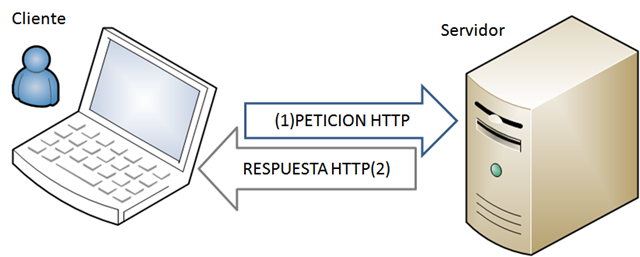
\includegraphics[width=0.5\linewidth]{Figures/Cliente_Servidor}
\decoRule
\caption[Esquema Cliente-Servidor]{Esquema Cliente-Servidor.}
\label{fig:Cliente_Servidor}
\end{figure}

Existen aplicaciones como los webmails figura \ref{fig:Gmail} , wikis figura \ref{fig:Wikipedia},
weblogs, tiendas en línea, que son ejemplos bien conocidos de aplicaciones web.

\begin{figure}[!h]
\centering
\subfigure[]{\label{fig:Gmail}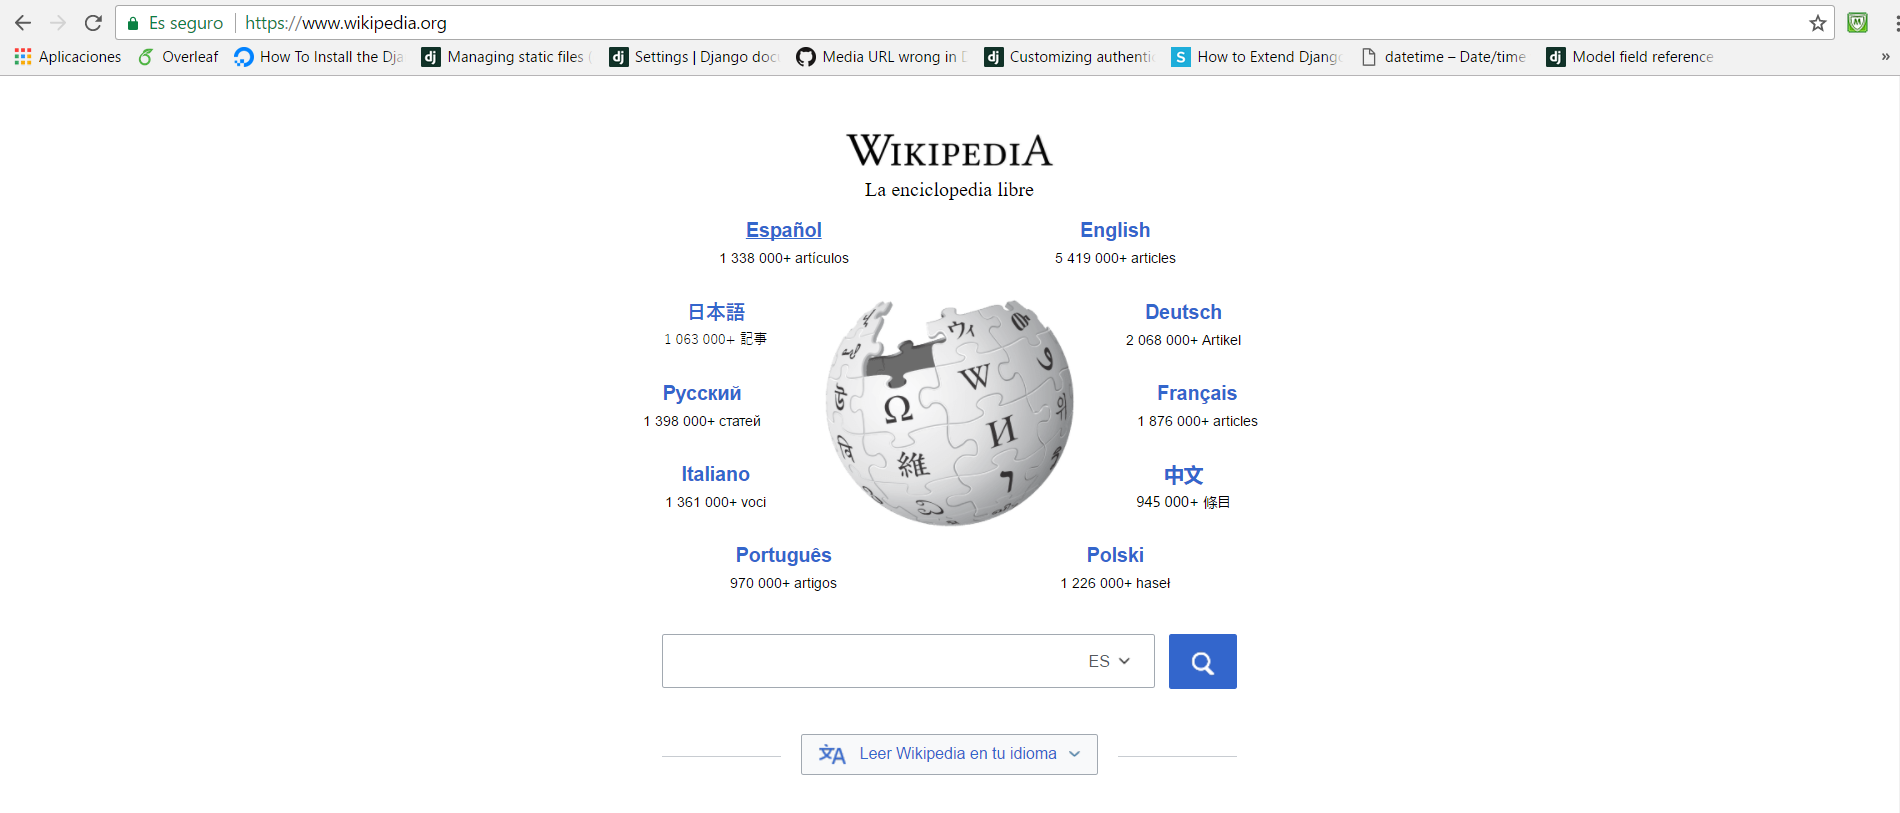
\includegraphics[width=0.9\linewidth]{Figures/wikipedia}}
\subfigure[]{\label{fig:Wikipedia}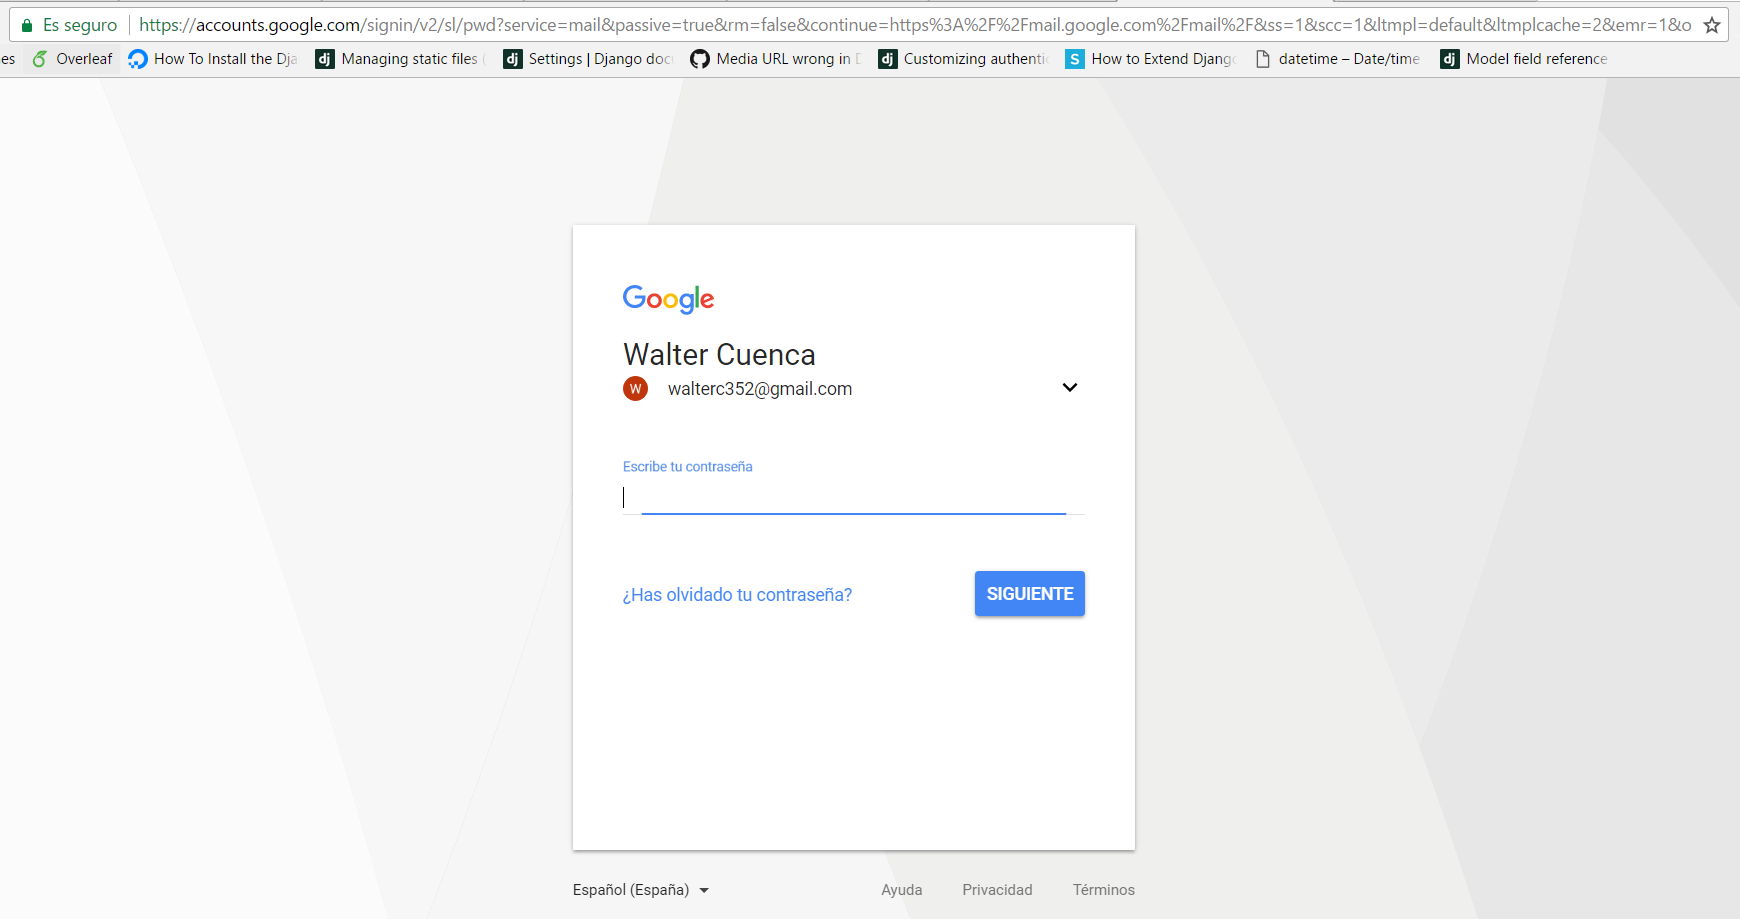
\includegraphics[width=0.9\linewidth]{Figures/gmail}}
\caption{Portada Wikipedia (a) y Portada Gmail (b)}
\end{figure}

Es importante mencionar que una página Web puede contener elementos que
permiten una comunicación activa entre el usuario y la información. Esto permite
que el usuario acceda a los datos de modo interactivo, gracias a que la página
responderá a cada una de sus acciones.
%,como por ejemplo rellenar y enviar
%formularios, participar en juegos diversos y acceder a gestores de base de datos
%de todo tipo.

La tendencia actual es la integración de medios digitales cuya información se encuentra almacenada digitalmente (texto,
gráficos, animación, voz y vídeo) que se combinan en la computadora para formar una única presentación. La utilización de los medios de esta forma permite crear entornos de comunicación mas participativos incrementando la eficiencia de la comunicación con el usuario final ya que combina información de varias fuentes 
\begin{figure}[!h]
\centering
\subfigure[]{\label{fig:Netflix}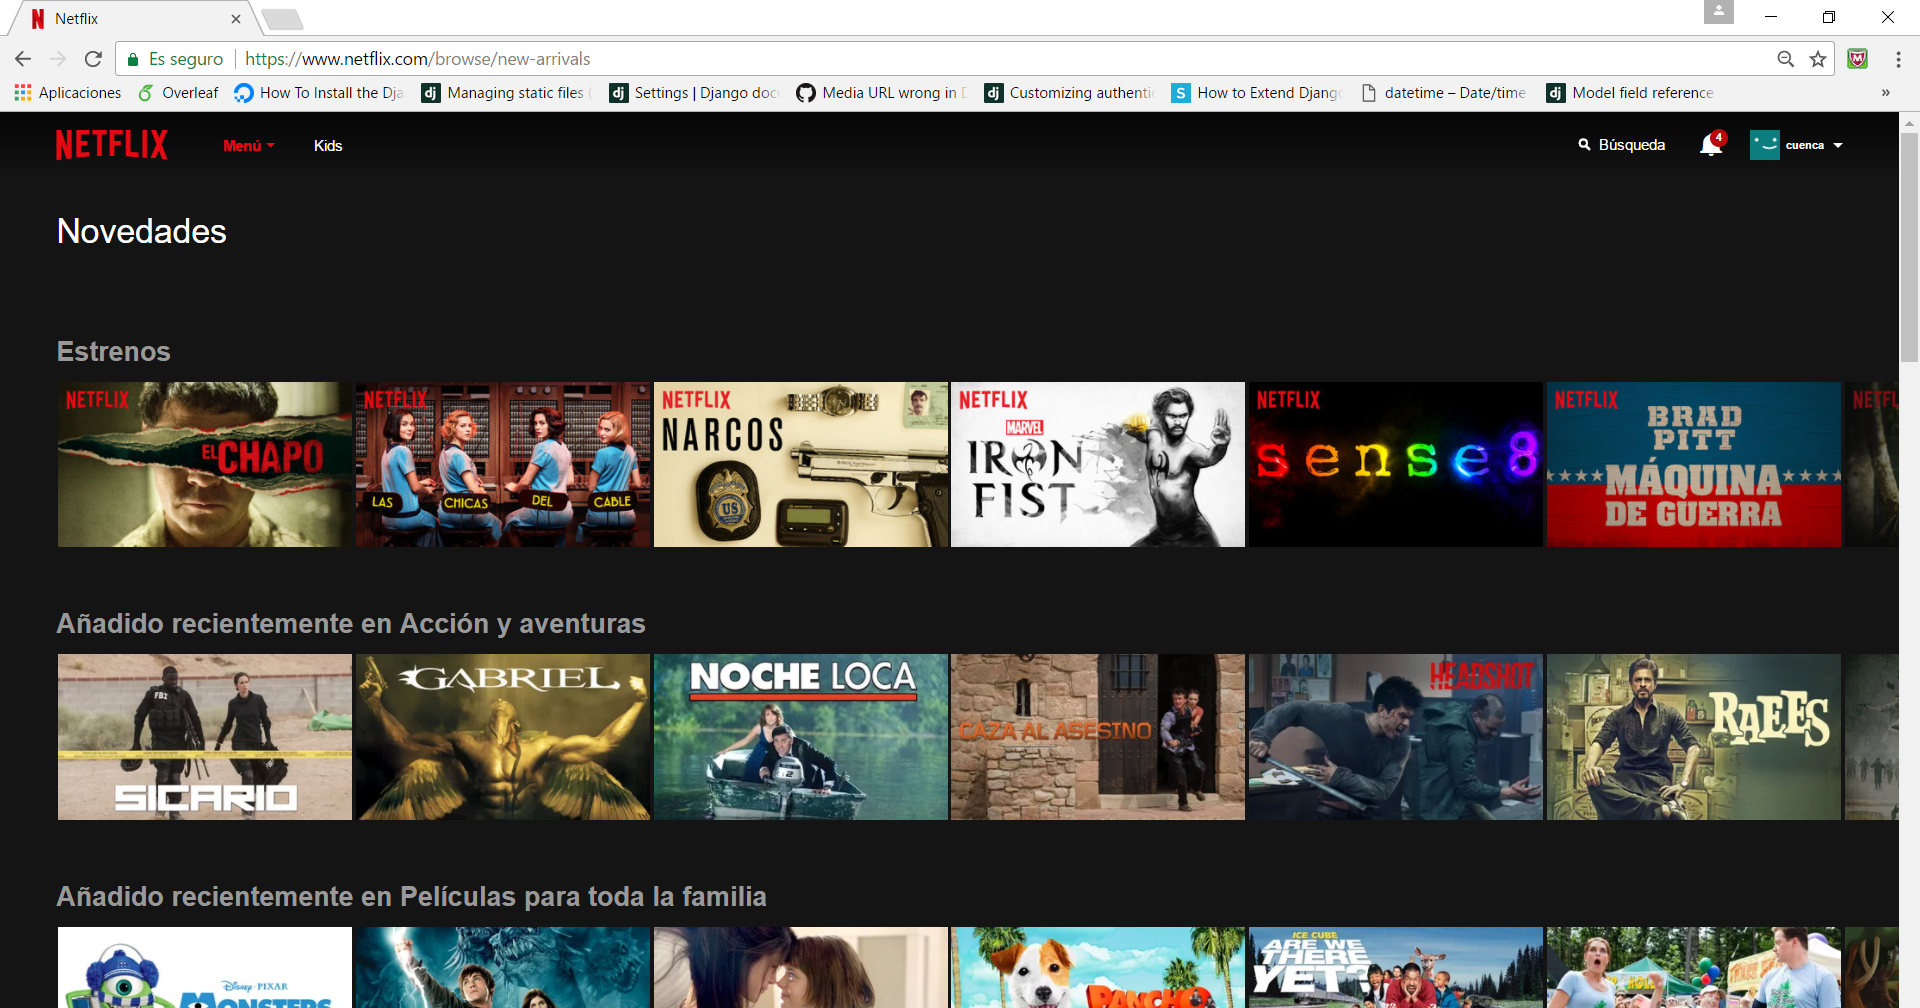
\includegraphics[width=0.9\linewidth]{Figures/netflix}}
\subfigure[]{\label{fig:YouTube}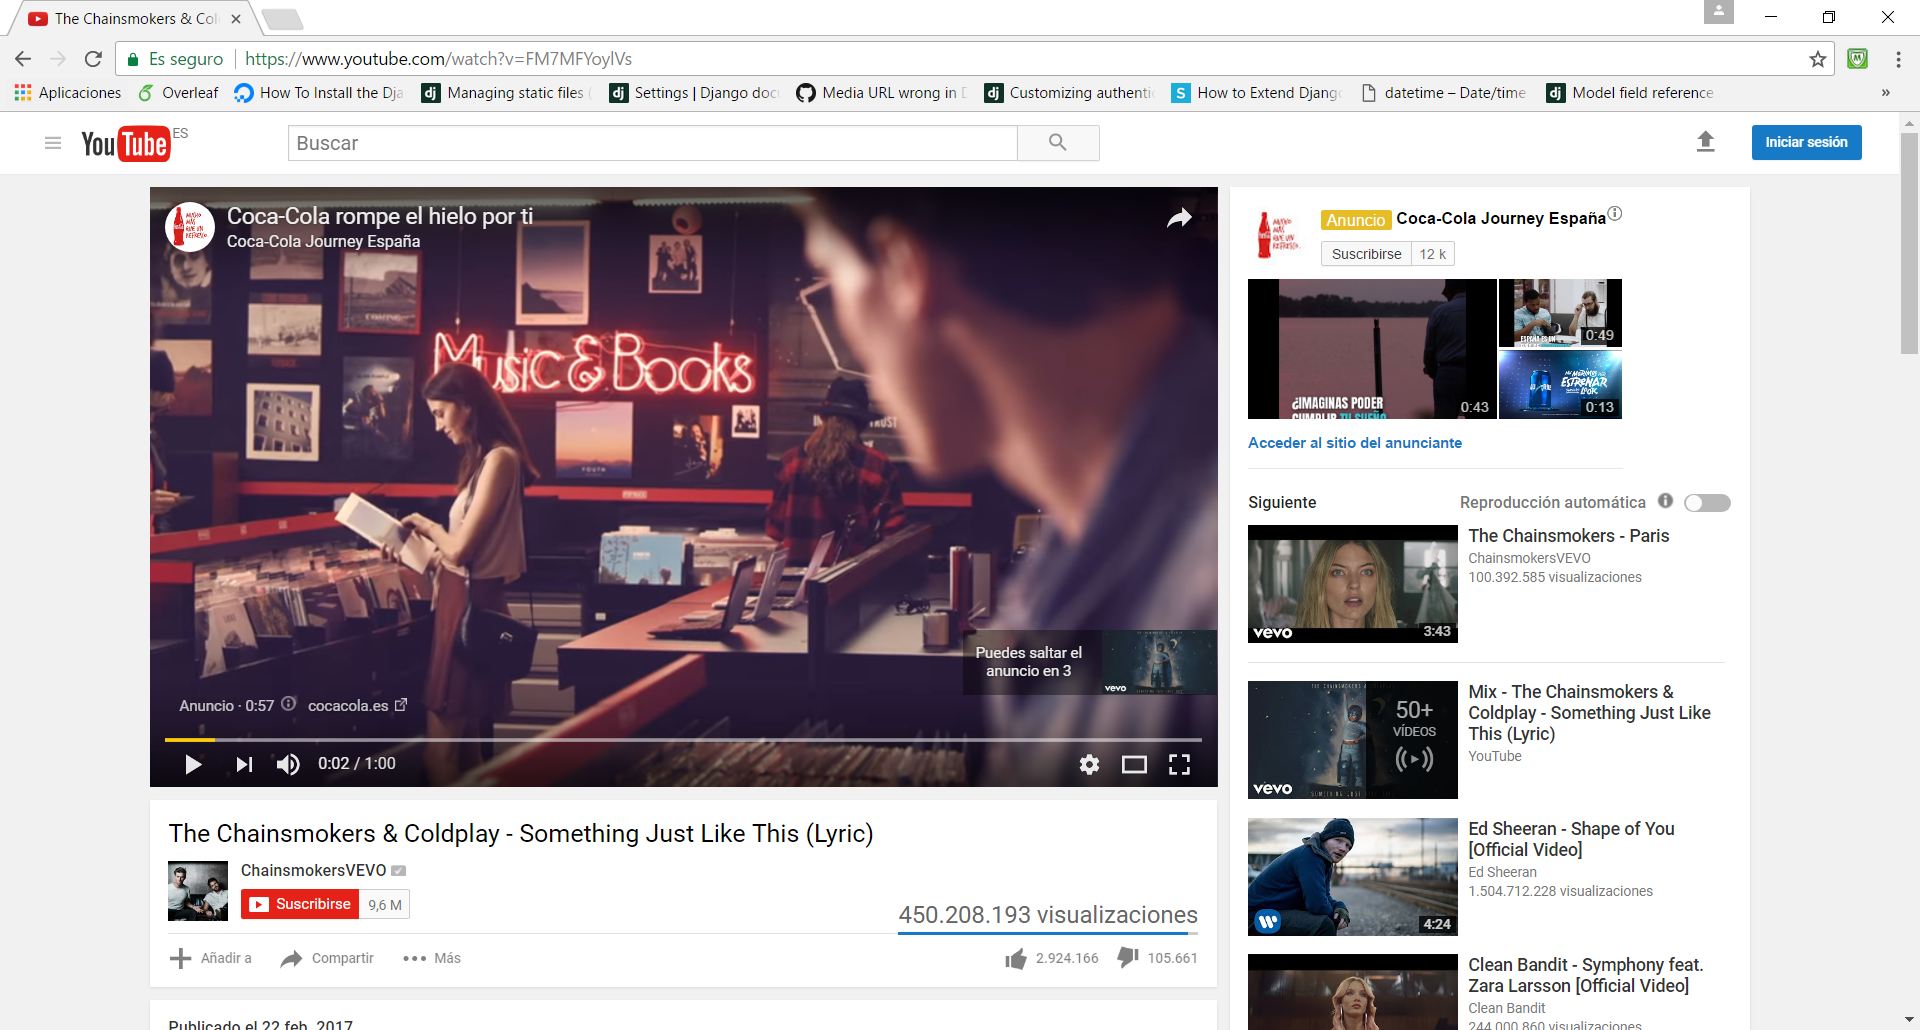
\includegraphics[width=0.9\linewidth]{Figures/YouTubePlay}}
\caption{Contenido Netflix (a) y Contenido YouTube (b)}
\end{figure}

%Multimedia: también denominada integración de medios digitales, consiste en un
%sistema que utiliza información almacenada o controlada digitalmente. La multimedia se pude definir, como una combinación de
%informaciones de naturaleza diversa, coordinada por la computadora y con la que
%el usuario puede interactuar. Se podrá emplear para realzar y optimizar el flujo de
%información, incrementando la eficacia de la comunicación entre el usuario final y
%la computadora.
%La utilización de medios digitales de forma interactiva permitirá crear un entorno de
%comunicación más participativo, ya que combina información de diversos medios 
%Índice
%Licenciatura en Sistemas de Información 61
%en una única corriente de conocimiento, aumentando el impacto que se produciría
%en los usuarios si se emplea de manera separada, los medios digitales que se
%incluyen en una computadora son Animación, Gráficos, Sonido y Vídeo
\section{Tecnologías Web}
\subsection*{Protocolo HTTP}
HTTP (\textit{Hyper Text Transfer Protocol}) ws un protocolo sin estado desarrollado por el \textit{World Wide Web Consortium} y la \textit{Internet Engineering Task Force}. Se compone de dos mensajes, el primer mensaje lo crea el cliente y es el requerimiento inicial de la comunicación. Este requerimiento llamado \textit{Request} esta dividido en una cabecera con la información de la pagina solicitada además de la aplicación cliente utilizada en el campo \texttt{User-Agent} y un mensaje de texto.
\begin{lstlisting}[
caption=Peticion HTTP.]
 GET /index.html HTTP/1.1
 Host: www.example.com
 User-Agent: HTTPTool/1.0
 Connection: close
 Linea en blanco
\end{lstlisting}
Una vez recibido el requerimiento el servidor devuelve una respuesta llamada \textit{Response} la cual también esta compuesta por una cabecera y un mensaje.
\begin{lstlisting}[
caption=Respuesta HTTP.]
 HTTP/1.1 200 OK
 Date: Fri, 31 Dec 2003 23:59:59 GMT
 Content-Type: text/html
 Content-Length: 1221
 <html><body>
 <h1>Pagina principal</h1></body></html>
\end{lstlisting}
\subsection*{HTML}
Son las iniciales de la expresión en inglés \textit{HyperText Markup Language}. Se trata de un conjunto de etiquetas que se van intercalando entre el texto de forma que los navegadores sepan qué es lo que tienen que mostrar cuando accedemos a una página y cómo deben presentarlo en la pantalla.

El W3C \footnote{Web: \url{http://www.w3.org/}} (World Wide Web Consortium) es el fórum internacional que se encarga desarrollar nuevas tecnologías relacionadas con la Web dictando las normas que constituyen el estándar HTML entre otros. A lo largo de sus diferentes versiones, se han incorporado y suprimido diversas características, con el fin de hacerlo más eficiente y facilitar el desarrollo de páginas web. La versión mas extendida fue la 4.0 que permitía utilizar textos, sonidos, imágenes y enlaces a otras páginas enriqueciendo de esta forma la información de la pagina.

A medida que este lenguaje se extendía se vio la necesidad de actualizar la versión del estándar. Es aquí, donde surge HTML5 \footnote{\url{http://www.w3.org/TR/2014/REC-html5-20141028/.}} que pretende cubrir varias necesidad que habían surgido hasta el momento. Dentro de estas nuevas características destacamos:
\begin{itemize}
\item \textbf{Contenido multimedia:} Habilita la posibilidad de incluir contenido multimedia de forma nativa sin necesidad de plugins o software de terceros.
\item \textbf{Animación:} Incluye nuevos elementos que permite crear contenido 2d y 3d dentro de la web.
\item \textbf{Comunicación:} Con la aparición de aplicaciones en tiempo real, era necesario proveer de mecanismos que permitan intercambiar datos de forma ligera y rápida. 
\end{itemize}
\section{Antecedentes}
El TFG centra su desarrollo en el campo de las tecnologías Web y como a través de ella permiten generar diversas aplicaciones con las que el usuarios pueden interactúar. Algunos trabajos previos existentes en los que se emplean estas tecnologías son los siguientes.
\subsection*{Surveillance 5.1 (URJC)}
Surveillance 5.1 \cite{TFGsurveillance5.1}\cite{surveillance5.1} fue desarrollado por Edgar Barrero como trabajo fin de grado. La aplicación web ofrece un flujo de vídeo desde una cámara web, un flujo de imagen de profundidad procedente de un sensor Kinect y su representación en 3D, además de un sensor de humedad y un actuador.

La aplicación web se desarrollo en Ruby on Rails. El servidor de la aplicación se conectaba a los componentes de JdeRobot a través del interfaz ICE.
\begin{figure}[!h]
\centering
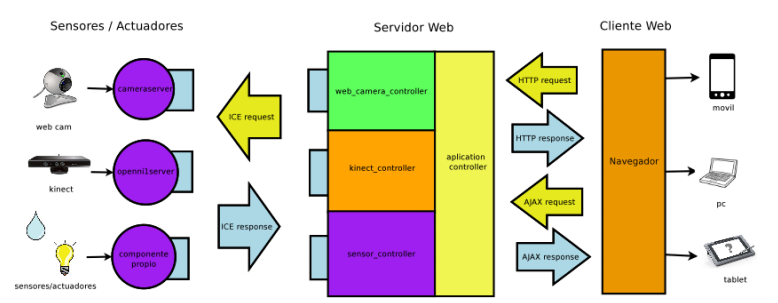
\includegraphics[width=0.5\linewidth]{Figures/edgar_surveillance_esquema}
\decoRule
\caption[Esquema Surveillance 5.1]{Esquema Surveillance 5.1.}
\label{fig:edgar_surveillance_esquema}
\end{figure}
\begin{figure}[!h]
\centering
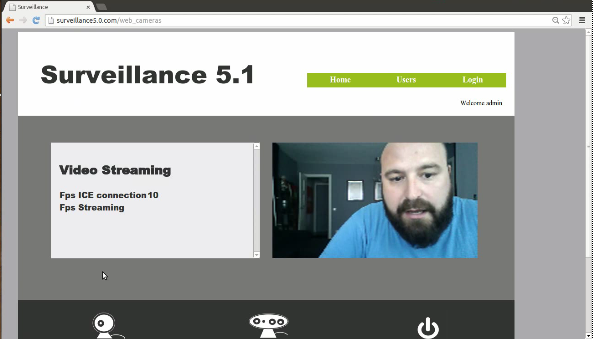
\includegraphics[width=0.5\linewidth]{Figures/edgar_surveillance5_web}
\decoRule
\caption[Interfaz Surveillance 5.1.]{Interfaz Surveillance 5.1.}
\label{fig:edgar_surveillance5_web}
\end{figure}
\subsection*{JdeRobotWebClients (URJC)}
JdeRobotWebClients \cite{TFGJdeRobotWebClients}\cite{JdeRobotWebClients} fue desarrollado por Aitor Martınez Fernandez como trabajo fin de grado. La aplicación Web crear seis versiones web de herramientas utilizadas por  JdeRobot (CameraViewJS, RGBDViewerJS, KobukiViewerJS, .....) que estaban programadas en C++ o Python con su propio interfaz gráfico provocando que sean ejecutables solo en Linux. 

Estas nuevas versiones pretenden ser multiplaforma (Linux, Android, IOS, Windows) y accesibles desde un navegador web como interfaz gráfico permitiendo acceder a los sensores y actuadores sin un servidor intermedio.
\begin{figure}[!h]
\centering
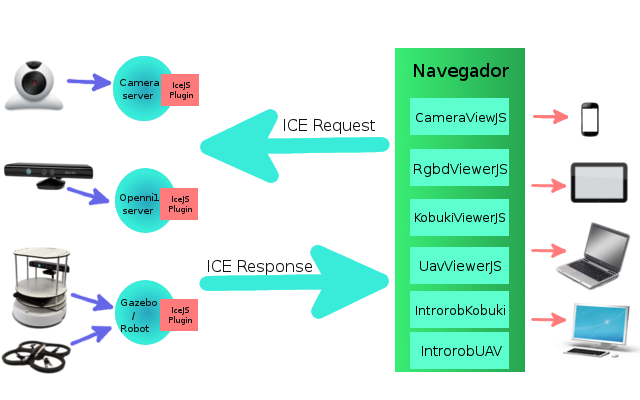
\includegraphics[width=0.5\linewidth]{Figures/Aitor_esq_proyecto}
\decoRule
\caption[Esquema JdeRobotWebClients]{Esquema JdeRobotWebClients.}
\label{fig:Aitor_esq_proyecto}
\end{figure}
\begin{figure}[!h]
\centering
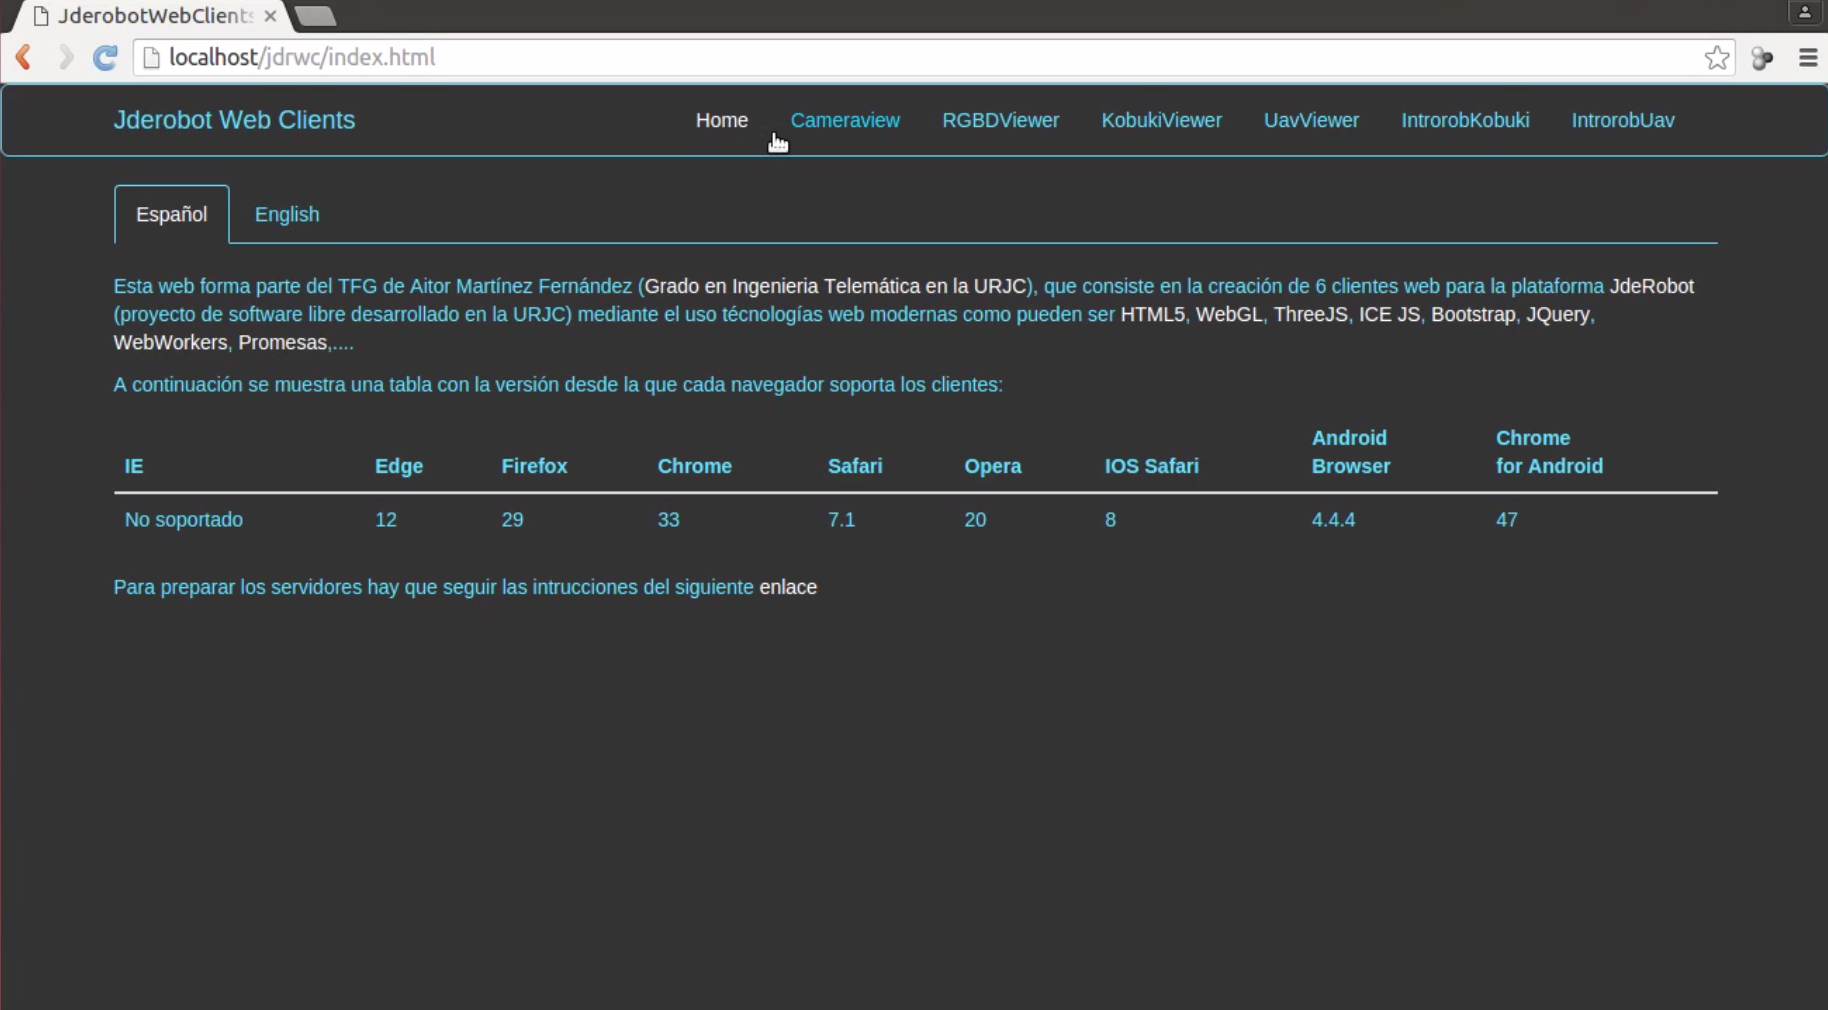
\includegraphics[width=0.5\linewidth]{Figures/Aitor_esquema_web}
\decoRule
\caption[Interfaz JdeRobotWebClients]{Interfaz JdeRobotWebClients.}
\label{fig:Aitor_esquema_web}
\end{figure}
\subsection*{Drone con WebRTC.}
Drone con WebRTC \cite{TFGDronWebRTC}\cite{DronWebRTC} fue desarrollado por Iván Rodríguez como trabajo de fin de grado. El objetivo era poder teleoperar un drone desde un dispositivo móvil (teléfono, tablets....) por medio de aplicaciones Web.

Su desarrollo se basaba en WebRTC como tecnología Web que para teleoperar el dron, además de emplear las tecnologías propias de Jderobot para establecimiento de conexión entre el dron y los dispositivos móviles.
\begin{figure}[!h]
\centering
\includegraphics[width=0.5\linewidth]{Figures/esquema_general_Ivan}
\decoRule
\caption[Esquema Dron con WebRTC]{Esquema Dron con WebRTC}
\label{fig:esquema_general_Ivan}
\end{figure}
\begin{figure}[!h]
\centering
\includegraphics[width=0.5\linewidth]{Figures/interfazweb_Ivan}
\decoRule
\caption[Interfaz Dron con WebRTC]{Interfaz Dron con WebRTC}
\label{fig:interfazweb_Ivan}
\end{figure}